\chapter{Architektur \textnormal{\textsf{\small{Jan Oehlers}}}}
\section{Einleitung}
Für die Entwicklung eines Planspiels sind grundlegende Rahmenbedingungen und Berechnungsvorschriften festzulegen. Diese basieren auf betriebswirtschaftlichen Überlegungen und realen Bestimmungen. Die Hauptanforderung an das Spiel ist eine möglichst genaue Widerspiegelung der Realität. Jeder Spieler übernimmt die Leitung über ein in Echtzeit simuliertes Unternehmen und muss sich mithilfe von strategischen und operativen Entscheidungen auf einem Oligopolmarkt gegen die anderen Mitspieler durchsetzen. Die Spieler leiten ihr Unternehmen für \enquote{10 Jahre} und 1 Quartal in Spielzeit entspricht einem \enquote{realen} Tag, dementsprechend dauert ein Spiel genau echte 40 Tage, sofern man nicht vorher bankrott geht. Die Konkurrenten auf dem Markt wechseln dauerhaft, da einige durch Bankrott ausscheiden, andere durch Ende ihrer Führungszeit beim Unternehmen, sowie jederzeit neue Spieler dem Markt beitreten können. Aufgrund von diesen schnellen Konkurrenzänderungen kann sich eine vermeintliche Marktführung innerhalb kürzester Zeit wieder aufheben oder wirklich schwache Unternehmen gewinnen deutlich an Marktmacht, weil die stärksten Konkurrenten ausscheiden. Dies impliziert, dass die Entscheidungen und der Erfolg anderer Unternehmen das eigene Unternehmen beeinflussen müssen. Dies wird zum Beispiel umgesetzt bei dem \enquote{Kampf} um Aufträge, da es sich bei unserem Markt um einen Business to Business Verkauf von Outdoor Artikeln handelt und von daher alle Aufträge als öffentliche Ausschreibungen ausgeschrieben werden kann jeder der Spieler, die derzeit auf dem Markt sind sich auf die Ausschreibung bewerben.

In diesem Kapitel werden zunächst die allgemeinen betriebswirtschaftlichen Aspekte, auf denen das Unternehmensplanspiel beruht, beleuchtet. Weiterhin werden die Funktionen der einzelnen Abteilungen, sowie der Mitarbeiter die dieser unterstellt sind erläutert und die Kennzahlenberechnung offengelegt, sowie deren Wechselwirkungen begründet. In Kapitel \ref{Jahresabschluss} auf S.\pageref{Jahresabschluss}  wird der Jahresabschluss bestehend aus Bilanz und Gewinn- \& Verlustrechnung, sowie die für dieses Planspiel relevanten Positionen betrachtet. 

\section{Betriebswirtschaftliche Aspekte}
\subsection{Branche}
Alle Unternehmen des Planspiels sollen einer Branche zugeordnet sein. In unserem Beispiel handelt es sich, wie vorher bereits erwähnt, um einen Business to Business Markt, bei dem alle Unternehmen Outdoor Artikel, um genauer zu sein Rucksäcke, Technische Funktionsrucksäcke, Duffels (eine Art Outdoor Reisetasche) und normale Reisetaschen herstellen. Es handelt sich um eine klassische, sowie auch moderne Produktionsindustrie, bei der weiterhin auch Forschung und Weiterentwicklung der eigenen Produktion eine wichtige Rolle spielt um sich langfristig auf dem Markt zu halten. Unsere Simulation beschränkt sich auf die reine Herstellung und den Vertrieb der Produkte, sodass die Rohstoffbeschaffung keine Rolle spielt. Es gibt alle vier verschiedenen eben erwähnten Produkte in drei unterschiedlichen Qualitätsstufen; A (\enquote{luxury}), B (\enquote{ordinary}) und C ({cheesy}) mit jeweils festgelegten Produktionskosten, welche die benötigten Rohstoffe beinhalten. Diese Kosten können durch die Erforschung neuer Produktionsverfahren verringert werden. 

Es werden durchgehend öffentliche Ausschreibungen generiert, auf die sich alle Spiele bewerben können mit zufälliger Auswahl des gewünschten Produktes, sowie einer zufällig generierten Menge von diesem Artikel, der auf der Durchschnittsproduktion aller Unternehmen basiert. Auf die genaue Entscheidung welcher Bewerber den Deal gewinnt, wird im weiteren Verlauf dieses Kapitels eingegangen. Jedes Unternehmen beginnt mit einem Eigenkapital von 100.000 \€. Um mit der Produktion anzufangen, muss zuerst ein Lager gekauft werden, um die hergestellten Produkte zu verstauen. Weiterhin muss eine Produktionshalle, in der Maschinen aufgestellt werden können, sowie eine Produktionsmaschine, speziell für ein bestimmtes Produkt angeschafft werden. Wer hier schon Fehleinkäufe macht und sich nicht auf die derzeitige Nachfragesituation auf dem Markt anpasst, ist schon prädestiniert schnell bankrott zu gehen. Danach muss man noch mindestens einen Mitarbeiter in der Abteilung Produktion einstellen, der die Maschine bedient um die Herstellung zu beginnen. Zusätzlich sollte man Mitarbeiter im Bereich des Vertriebs einstellen um sich auf Ausschreibungen bewerben und diese gewinnen zu können, da man ansonsten auf Lager produziert ohne einen Abnehmer zu besitzen. 

\section{Kennzahlen}
Der Erfolg der einzelnen Unternehmen wird anhand von verschiedensten sich gegenseitig beeinflussenden Kennzahlen bemessen. Diese nehmen, zumindest für die \enquote{weichen} Kennzahlen \%-Werte zwischen 0 und 100 an. Zu diesen Kennzahlen zählen der Marktanteil, die Mitarbeiterzufriedenheit, die Kundenzufriedenheit, das Image des Unternehmens, der Bekanntheitsgrad, sowie die Verkaufswahrscheinlichkeit, also die Chance einen Deal zu gewinnen auf den man sich beworben hat. Diese weichen Kennzahlen, werden (abgesehen von dem Marktanteil, da dieser ein reines Verhältnis widerspiegelt) jedes Quartal um 1\% gesenkt, da wenn man sich auf dem Markt für längere aus der Werbung zum Beispiel wieder raushält, der eigene Bekanntheitsgrad nachlässt. Einige dieser Kennzahlen werden mithilfe den Werten andere Kennzahlen berechnet oder berechnen sich einfach aus Daten des Unternehmens, wie der Marktanteil zum Beispiel, welcher sich rein aus den verkauften Produkten der Unternehmen berechnet. Weiterhin ist es möglich alle diese Kennzahlen durch bestimmte Aktionen im Spiel zu beeinflussen und so seine Gewinnchancen zu erhöhen, welche im später folgenden Kapitel über die Abteilungen genauer erläutert werden. Weiterhin gibt es einige \enquote{harte} Kennzahlen, welche beliebig hohe \€-Beträge annehmen können und hier in Form der Positionen in der Bilanz, sowie der Gewinn- und Verlustrechnung auftreten.

Alles weichen Kennzahlen werden in eine hyperbolische Funktion eingesetzt, um eine möglichst realitätsgetreue Entwicklung der Kennzahlen zu modellieren. Durch diese werden \%-Werte zwischen 2 und 98 als Maximalwert angenommen, da eine Kundenzufriedenheit von genau 100\% utopisch wäre. Außerdem wird dadurch der gerade Verlauf der Variablen angepasst, wodurch die Kennzahlen erst schwach ansteigen, dann ab einem Standard-Wert von ca. 0.4 stark steigen und sich dann schwach an 100\% annähern, diese jedoch nie erreichen, da ab einem bestimmten Wert einer Kundenzufriedenheit zum Beispiel es nur sehr schwer ist, diese weiterhin stark zu erhöhen. Der in unserem Projekt verwendete Tangens Hyperbolicus entspricht der Funktion y= 0.5 * tanh(4x-2) + 0.5, dessen Verlauf in Grafik \ref{hyperbolic_function} sichtbar ist und von Java in dieser Form schon unterstützt wird.
\begin{figure}
	\centering
	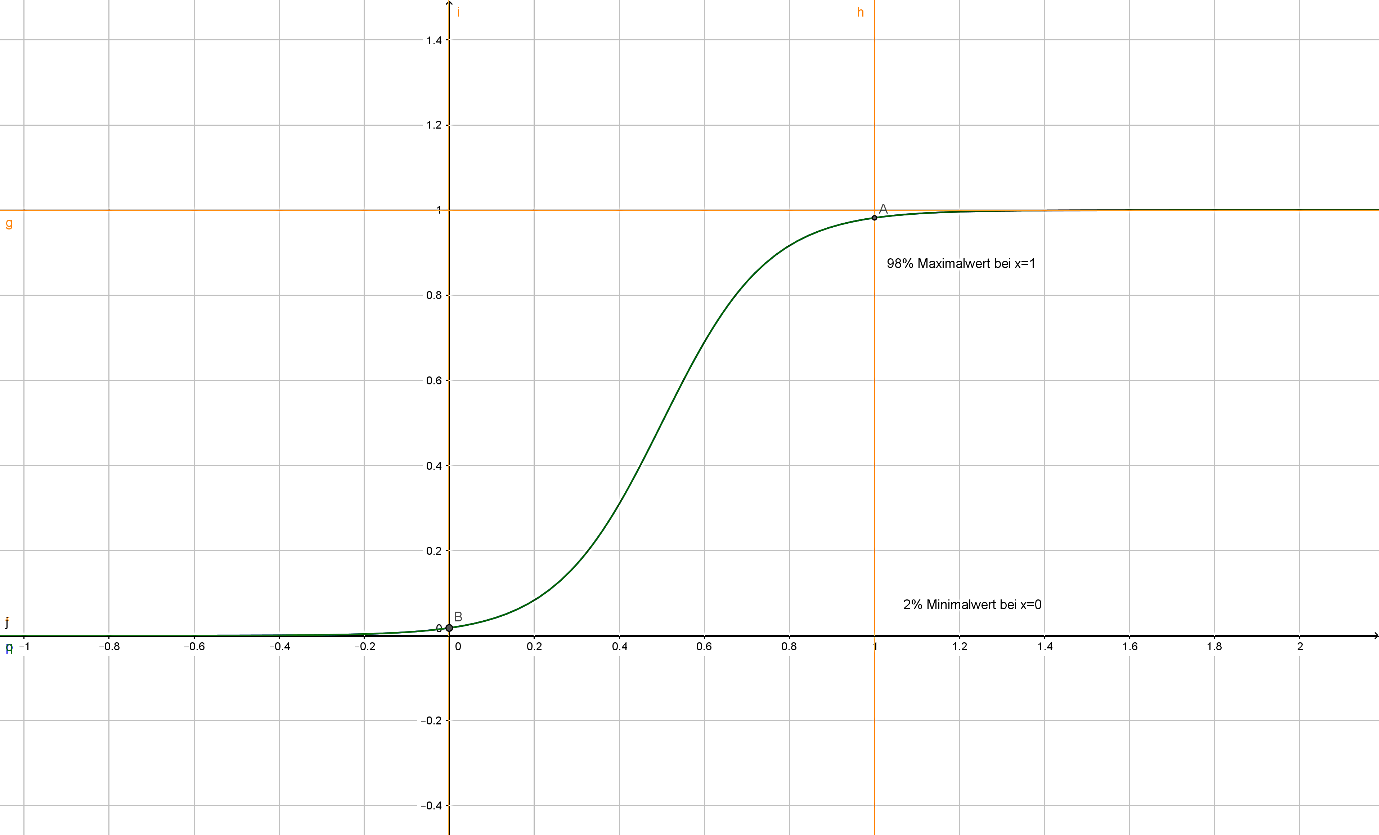
\includegraphics{Funktion.png}
	\caption{Grafik der Hyperbolischen Funktion}
	\label{hyperbolic_function}
\end{figure}

Im folgenden wird nun die Berechnung der Kennzahlen, sowie deren genauer Einfluss offen gelegt.  

\subsection{Marktanteil} 
Der Marktanteil eines Unternehmens zählt zur Kategorie der weichen Kennzahlen und berechnet sich einfach aus dem Verhältnis der eigenen verkauften Produkte, zu den verkauften Produkten aller Unternehmen. Diese wird dabei nicht durch die hyperbolische Funktion angepasst, da diese Kennzahl ein reines Verhältnis widerspiegelt. Des weiteren wird nicht zwischen den einzelnen Kategorien der Artikel, also ob Duffel oder Rucksack o.ä. unterschieden, da es sich um einen großen gemeinsamen Markt (den der Outdoor \enquote{Accessoires}) handelt. Dies bedeutet auch, dass wenn sich plötzlich viele neue Spieler anmelden, der eigene Marktanteil drastisch senken kann. 

Der Marktanteil besitzt keine weiterführenden Wechselwirkungen, sondern ist nur ein Indikator, wie sich das Unternehmen im Vergleich zu den anderen schlägt. Dadurch, dass die Verkaufswahrscheinlichkeit zum Großteil bestimmt, ob man Deals gewinnt und diese dann den Marktanteil bestimmen, ist es wichtig eine möglichst hohe Verkaufswahrscheinlichkeit zu besitzen um möglichst viele Deals für sich zu gewinnen, wenn man seinen Marktanteil maximieren möchte. 

\subsection{Mitarbeiterzufriedenheit}
Die Mitarbeiterzufriedenheit des Unternehmens berechnet sich aus dem Durchschnittsgehalt aller Mitarbeiter die im Unternehmen angestellt sind. Dieses wird durch einen festgelegten Wert geteilt, der benötigt wird um eine 100-prozentige Zufriedenheit der Mitarbeiter nur auf Basis ihres Gehaltes zu gewährleisten. Dieser Wert entspricht bisher 70.000\€ jährlich, da dies ein angemessener Durchschnittswert für alle Mitarbeiter, also auch die, die nur in der Produktion arbeiten, sowie für die normalerweise besser verdienenden Sales-Leute, ist, um eine volle Zufriedenheit zu erreichen. Diese kann auch durch soziale Leistungen, wie zum Beispiel dem Aufbau einer Kantine erhöht werden, sodass ein Durchschnittsgehalt von 70.000\€ nicht zwingend notwendig ist um eine vollständige Zufriedenheit der Mitarbeiter sicherzustellen. 

Eine hohe Mitarbeiterzufriedenheit hat vielerlei positive Auswirkungen auf das Unternehmen. Sie erhöht zum Beispiel die Produktivität der Mitarbeiter in der Produktion, von daher können mit derselben Anzahl Mitarbeiter mehr Produkte im Monat hergestellt werden. Außerdem bestimmt sie das Image, wodurch indirekt die Verkaufswahrscheinlichkeit erhöht wird und verkürzt die Dauer der Forschungsprojekte, da zufriedenere Mitarbeiter einfach effektiver arbeiten. 
\subsection{Kundenzufriedenheit}
Die Kundenzufriedenheit startet immer bei 0\% und lässt sich durch Forschungsmaßnahmen erhöhen. Diese geben den Produkten sozusagen neue Alleinstellungsmerkmale, die den Kunden glücklicher mit dem erworbenen Produkt werden lassen. Dies ist der einzige Weg seine Kunden zufrieden zu stellen, jedoch sinkt die Kundenzufriedenheit, wenn man gewonnene Deals nicht erfüllt, mal abgesehen von dem Verlust durch Konventionalstrafen (mehr dazu später), sowie wie die anderen weichen Kennzahlen auch in bestimmten Zeitabständen.

Die Kundenzufriedenheit spielt eine wichtige Rolle für das Image, welches neben dem Bekanntheitsgrad der ausschlaggebende Faktor in der Verkaufswahrscheinlichkeit, das heißt sie spielt auch eine relativ wichtige Rolle in dem Erfolg des Unternehmens, da Produkte verkaufen der einzige Weg Umsatz zu erzielen ist.  
\subsection{Image}
Das Image eines Unternehmens ist das generelle Bild welches Externe, also Kunden, sowie andere Unternehmer von der Firma haben. Dieses ist die erste hier aufgeführte Kennzahl, die sich nur aus anderen zuvor erklärten Kennzahlen berechnet. Sie wird zur einen Hälfte aus der Mitarbeiter- und zur anderen Hälfte der Kundenzufriedenheit berechnet, da zufriedene Mitarbeiter oder Kunden positiv von dem Unternehmen sprechen, wodurch sich das Image verbessern könnte. Außerdem haben Unternehmen von denen generell die Mitarbeiter und Kunden alle Unzufrieden sind es eher schwerer ein positives Image in der Öffentlichkeit zu bewahren. 
Das Image beeinflusst die Verkaufswahrscheinlichkeit und kann auch durch soziale Projekte, wie zum Beispiel Spenden erhöht werden.
\subsection{Bekanntheitsgrad}
Der Bekanntheitsgrad wird ähnlich wie die Kundenzufriedenheit nicht berechnet, sondern startet auch bei 0\% und erhöht sich nur durch Aktionen in der Marketing Abteilung. Er ist neben dem Image der Hauptfaktor für die Verkaufswahrscheinlichkeit, von daher ist es sehr empfehlenswert in irgendeiner Art Marketing Maßnahmen durchzuführen. 
\subsection{Verkaufswahrscheinlichkeit}
Die Verkaufswahrscheinlichkeit ist wahrscheinlich die Kennzahl mit dem größten Einfluss auf den Erfolg des Unternehmens, da es mit einer schlechten Verkaufswahrscheinlichkeit fast unmöglich ist irgendwelche Deals zu gewinnen und außerdem eine hohe Verkaufswahrscheinlichkeit auch die Erträge aus Deals erhöht. Da diese die einzige Möglichkeit sind Gewinne zu erzielen sollte man unbedingt eine hohe Verkaufswahrscheinlichkeit anstreben. Diese wird zu 50\% aus dem Image und zu den anderen 50\% aus dem Bekanntheitsgrad gerichtet, also sollte das Hauptziel jedes Unternehmers sein diese zu maximieren. Dies ist in der Realität fundiert, da ein vollkommen unbekanntes Unternehmen nur schwer Deals gewinnen kann, da niemand \enquote{No-Name} Produkte kauft. Des weiteren ist es vor allem auf einem Markt, wie dem der Outdoor Artikel sehr schwer Käufer zu finden wenn das Unternehmen ein sehr negatives Image hat, da die Käufer besonders großen Wert auf Qualität legen und lieber mehr zahlen, als zu wissen, dass ihre Produkte unter sehr schlechten Arbeitsbedingungen, zum Beispiel, hergestellt werden. 

\section{Absatz der Produkte}
Es werden durchgehend öffentliche Ausschreibungen generiert, deren Anzahl mit der Anzahl an aktiven Spielern auf dem Markt skaliert, das heißt gibt es mehr Bewerber, werden logischerweise auch mehr Ausschreibungen erstellt. Für diese hat nun jeder Spieler einen Monat (in Spielzeit), also in etwa 8 Stunden um sich darauf zu bewerben, bevor eine Entscheidung für ein Unternehmen getroffen wird. Wer aktiv ist und sich zuerst bewirbt hat eine theoretisch höhere Chance die Ausschreibung für sich zu entscheiden als spätere Bewerber, denn am Entscheidungstag wird eine Zufallszahl zwischen 0 und 1 erstellt und mit der Verkaufswahrscheinlichkeit des ersten Bewerbers verglichen. Ist die Kennzahl höher als die erzeugte Zufallszahl wird der Deal gewonnen, falls nicht wird dieselbe Rechnung mit dem nächsten Bewerber durchgeführt, bis ein Unternehmen die Ausschreibung für sich entscheidet, oder kein Bewerber mehr über ist. 

Die geforderten Produkte in den Ausschreibungen werden zufällig erstellt, sowie die Menge, jedoch im Verhältnis zur Durchschnittsproduktion aller Unternehmen und die Laufzeit variiert auch zufällig, das heißt es können Aufträge für 1000 Rucksäcke jeden Monat 2 Jahre lang oder eine Einmal-Bestellung von 500 Duffels zum Beispiel erstellt werden. Ist ein Deal einmal gewonnen, kann dieser nicht mehr abgebrochen werden und Nichtlieferung führt zu Konventionalstrafen in Höhe von 75\% des Preises. Dieser wird nach Gewinn des Deals berechnet, da die Kennzahl Verkaufswahrscheinlichkeit auch eine Rolle bei der Höhe des erzielten Gewinnes spielt, da Unternehmen mit einem besseren Image oder höherem Bekanntheitsgrad, höhere Preise erzielen können. 

\section{Jahresabschluss} \label{Jahresabschluss}
Nach dem Handelsgesetzbuch (HGB) sind alle Kaufleute verpflichtet, einen Jahresabschluss aufzustellen (vgl. § 242 HGB). Dieser besteht aus Bilanz und GuV, Kapitalgesellschaften müssen zusätzlich einen Anhang, sowie Lagebericht veröffentlichen. Der Jahresabschluss hat unter anderem eine Dokumentationsfunktion,gekennzeichnet durch eine laufende Buchführung, sowie eine Informationsfunktion.Letztere ermöglicht einen Überblick über die Vermögenslage (Mittelverwendung), die Finanzlage (Mittelherkunft) und die Ertragslage eines Unternehmens.
In unserem Planspiel werden in der Bilanz und der GuV nur die in diesem Spiel berührten Positionen aufgeführt, welche den beim Kennzahlenprinzip erwähnten \enquote{harten} Kennzahlen entsprechen. Einmal jährlich wird ein Jahresabschluss durchgeführt um die Bilanz auszugleichen. 
Im Spiel wird auch unterjährig eine nicht ausgeglichene Bilanz angezeigt, welche aber nicht zur Veröffentlichung, sondern nur zur Information des Spielers dient. Diese enthält die in diesem Spiel berührten Aktiv- und Passiv-Positionen: 
\begin{itemize}
\item \textbf{Aktiva}	
	\begin{itemize}
		\item Technische Anlagen und Maschinen
		\item Gebäude
		\item fertige Erzeugnisse
		\item liquide Mittel
	\end{itemize}
\item \textbf{Passive}
	\begin{itemize}
		\item Fremdkapital
		\item Eigenkapital
	\end{itemize}
\end{itemize}

Jeder Spieler beginnt mit einem Eigenkapital von 100.000€ und von daher auch mit liquiden Mitteln in der selben Höhe. Die restlichen Bilanzpositionen entsprechen erst einmal 0 und können zum Beispiel durch den Kauf von Produktionsmaschinen oder Lager- beziehungsweise Produktionshallen erhöht werden. Die fertigen Erzeugnisse werden direkt durch Produktion und dadurch Senkung der liquiden Mittel erhöht, da wir keine eigenen Rohstoffkonten haben und von daher direkt produziert wird wenn man Geld für die Herstellung ausgibt. Außerdem lassen sich die Liquiden Mittel durch Aufnahme von Krediten, also Fremdkapital aufstocken.

Die Gewinn- und Verlustrechnung erhält auch nur die Aufwands- und Ertragsposten die in unserer Simulation relevant sind und diese beschränken sich auf:
\begin{itemize}
	\item \textbf{Aufwendungen}	
	\begin{itemize}
		\item Aufwendungen für Rohstoffe
		\item Aufwendungen für Werbung
		\item Aufwendungen für Gehälter
		\item Aufwendungen für Energie
		\item Aufwendungen für soziale Leistungen
		\item Zinsaufwendungen
		\item Aufwendungen für Fremdinstandhaltung
		\item Schadensersatzzahlungen
		
	\end{itemize}
	\item \textbf{Erträge}
	\begin{itemize}
		\item Umsatzerlöse für fertige Erzeugnisse
		\item Jahresüberschuss
	\end{itemize}
\end{itemize}

Unsere GuV enthält alle Aufwandskonten die in unserer Simulation möglicherweise belastet werden könnten und außerdem das einzige Ertragskonto, die Umsatzerlöse, die wie schon mehrfach erwähnt wurde unsere alleinige Umsatzquelle sind. Der Jahresabschluss wird einmal jährlich aus den Umsatzerlösen - die kumulierten Aufwendungen berechnet und danach entweder dem Eigenkapital in der Bilanz zugerechnet (wenn die Erlöse höher sind als die Aufwendungen) oder vom Eigenkapital substrahiert, wenn er negativ ist. Dadurch erhält der Spieler einen guten Überblick über den Erfolgs des Unternehmens der letzten Quartale und erhält außerdem einen Indikator auf seine Chancen in der Highscore Liste zu landen, da dort das Eigenkapital übernommen wird, also der kumulierte Gewinn seiner 10 Jahre Spielzeit. 

\section{Abteilungen}
\subsection{Einführung}
Es gibt in diesem Planspiel sechs verschiedene Abteilungen, denen der Spieler Mitarbeiter zuordnen und in denen er freie Entscheidungen treffen kann. Diese Abteilungen, sowie die einzelnen Entscheidungsmöglichkeiten und deren Konsequenzen werden in diesem Kapitel erklärt. Außerdem wird die Funktion der Mitarbeiter, die den einzelnen Abteilungen unterstellt sind erläutert und die Hintergründe beleuchtet, warum man Mitarbeiter in bestimmten Abteilungen einstellen muss.
\subsection{Human Ressources}
Über die Abteilung Human Ressources ist es dem Spieler möglich neue Mitarbeiter einzustellen und deren Abteilung, sowie Gehalt zu bestimmen. Dieses ist vollkommen frei wählbar und daher sind dem Unternehmer alle Möglichkeiten offen eine bestimmte Führungsstrategie zu verfolgen, wie etwa Kostenführerschaft, durch möglichst geringe Gehaltszahlungen und Produktionskosten. Jedoch wirkt sich das Gehalt direkt auf die Mitarbeiterzufriedenheit und dadurch einige andere Kennzahlen des Unternehmens aus. Weiterhin lassen sich dort die derzeitigen Mitarbeiter einsehen und der Spieler kann soziale Projekte starten, wie zum Beispiel einen Kindergarten für die Mitarbeiterkinder eröffnen, freies WiFI einrichten, Urlaubs- oder Weihnachtsgeld zusätzlich ausbezahlen oder eine Kantine finanzieren. Dadurch erhöht sich die Mitarbeiterzufriedenheit deutlich, jedoch sind alle diese Leistungen auch mit monatlichen, beziehungsweise einmaligen Kosten verbunden. Außerdem ist für jeden 10. Mitarbeiter den man generell einstellen möchte, ein Mitarbeiter, der der Abteilung Human Ressources unterstellt ist notwendig, da man ab einer gewissen Größe des Unternehmens die Mitarbeiter nicht mehr alleine einstellen und verwalten kann. 

\subsection{Produktion}
In der Produktionsabteilung kann der Unternehmer, wie der Name schon sagt, Produkte herstellen. Dafür muss er eine Lager-, sowie Produktionshalle erwerben, mindestens einen Mitarbeiter in dieser Abteilung einstellen und eine Produktionsmaschine kaufen, für den Artikel den er gerne herstellen würde. Die monatliche Produktionsmenge kann vom Spieler in vorm von Produktlinien festgelegt werden, sofern die eben genannten Grundvoraussetzungen erfüllt sind. Die maximale Produktionsmenge pro Monat wird durch die Anzahl der Maschinen, welche hingegen vom Platz in der Produktionshalle beschränkt ist, und der Anzahl der Mitarbeiter festgelegt. Der niedrigere Wert von beidem bestimmt die Obergrenze, wobei die maximalen Produkte pro Monat pro Mitarbeiter durch eine hohe Mitarbeiterzufriedenheit erhöht werden kann, da sehr zufriedene Mitarbeiter mit den selben Maschinen mehr produzieren können, da sie weniger Fehler machen.

Der Spieler hat die Auswahl Produkte der drei verschiedenen Qualitätsstufen A, B und C herzustellen. Die jeweiligen Herstellungskosten basieren auf Einkaufskosten der verschiedenen Produkte von wirklichen Outdoorherstellern um die Hälfte reduziert, da in unserem Planspiel nur die Herstellungskosten gefordert sind und Aufwendungen wie Energie oder die Maschinen (die in den Kaufpreis logischerweise eingerechnet sind) oder Gewinnmargen noch heruntergerechnet werden müssen. 

Die Grundvorraussetzungen für die Produktion sind sehr komplex, jedoch von der Realität ableitbar, da man ohne Halle zum Beispiel nur schwer produzieren kann und die jeweiligen Funktionen zum Kaufen der einzelnen Bestandteile sehr offensichtlich in der Produktionsabteilung ersichtlich sind.

\subsection{Forschung}
Auf dem Outdoor Markt spielt die Weiterentwicklung der eigenen Produkte eine große Rolle um die eigene Marktpositionen zu stärken und dies kann man in der Abteilung Forschung durchführen. Es gibt zwei verschiedene Arten durchführbarer Forschungen, beide für alle verschiedenen Produktqualitätsstufen differenziert. Der Spieler kann die Kundenzufriedenheit seiner Produkte verbessern, indem er nach neuen Zusatzfeatures forscht, die das Erlebnis der Kunden mit dem Produkt besser machen und dadurch die Zufriedenheit erhöhen oder durch die Erforschung neuer Produktionsmethoden die Herstellungskosten für ein bestimmtes Produkt in einer bestimmten Qualitätsstufe senken, um sich so weiter auf eine bestimmte Produktion zu spezialisieren. Um eine Forschung durchführen zu können, muss mindestens ein Mitarbeiter in der Forschungsabteilung eingestellt werden und die Zeit die ein einziges Forschungsprojekt dauert, skaliert mit der Anzahl der Mitarbeiter die daran arbeiten, das heißt je mehr Mitarbeiter man in der Abteilung einstellt, desto schneller werden Forschungen abgeschlossen. Weiterhin beschleunigt werden diese durch zufriedene Mitarbeiter. 
Diese Abteilung stellt die einzige Möglichkeit dar, die Kundenzufriedenheit zu erhöhen und ist damit sehr relevant für die Verkaufswahrscheinlichkeit.

\subsection{Marketing}
In der Marketingabteilung kann der Unternehmer Marketingkampagnen starten um seine Produkte zu bewerben und so den Bekanntheitsgrad seines Unternehmens zu erhöhen, um die Chance Deals zu gewinnen zu steigern. Es gibt vier verschiedene Kampagnen mit unterschiedlichen Kosten und dementsprechenden benötigten Mitarbeitern um diese durchzuführen. Diese sind eine den Kosten nach aufsteigend sortiert \enquote{Sozial Media Kampagne}, \enquote{Werbung in Printmedien}, \enquote{Radiowerbespot} und \enquote{TV-Spot}. Die im Interface angezeigten Kosten werden täglich abgerechnet und entsprechen realen Kosten, für die Simulation der Kosten für einen TV-Spot zum Beispiel wurden einige Berechnungsannahmen getroffen. Die 130.000 \€ täglich setzen sich aus den generellen Sendekosten an den Sender (ca 60.000 pro Spot in der Prime-Time, je nach Sender) und den Produktionskosten für einen eigenen Spot zusammen. Diese werden nicht als direkte Fixkosten abgerechnet, sondern gehen in den täglichen Kosten auf. Weiterhin wird davon ausgegangen, dass der Spot zwei mal täglich in der \enquote{Prime-Time} gesendet wird, um so die größtmögliche Zielgruppe zu erreichen und dem Spieler, mit schon hohen Einnahmen eine Möglichkeit zu geben seine Verkaufsmöglichkeiten enorm zu erhöhen. Außerdem werden mindestens 7 Mitarbeiter in der Abteilung Marketing benötigt um einen Tv-Spot zu ermöglichen. 

\subsection{Finanzen}
Die Finanzabteilung bietet Einsicht in die vorher erklärte Bilanz und GuV des Unternehmens und gibt so dem Spieler einen Überblick über seinen Erfolg und seine laufenden Kosten. Außerdem bietet diese Abteilung die Möglichkeit Kredite aufzunehmen um so die Zahlungsmittel des Unternehmens zu erhöhen. Die Zinsen für den Kredit werden mithilfe der Verschuldungsquote, also Eigenkapital / Fremdkapital berechnet. Überschreitet diese zwei, hat man also doppelt so viel Fremdkapital wie eigenes ist es nicht mehr möglich neue Kredite aufzunehmen, da der Bank nicht genug Sicherheiten angeboten werden können, um einen neuen Kredit gewährt zu bekommen.

\subsection{Vertrieb}
In der Abteilung Vertrieb kann der Spieler die derzeit offenen Ausschreibungen sehen und sich darauf bewerben, außerdem werden die gewonnenen Deals mit Auftragsvolumen angezeigt, wodurch man sich einen Überblick darüber verschaffen kann, wieviel man diesen Monat produzieren muss um seine Verträge zu erfüllen. Jedes Unternehmen beginnt bei Erzeugung direkt mit einem zufällig generierten Auftrag, ohne Konventionalstrafe um dem Spieler direkt einen schnellen Start mit Aussicht auf Gewinne zu ermöglichen, ohne einen Monat nur zu produzieren und zu hoffen man gewinnt einen der ersten Deals. Des weiteren erfolgt in dieser Klasse die in diesem Kapitel erklärte Ausschreibungsgewinnermittlung. Um sich auf neue Ausschreibungen bewerben zu können, muss man mindestens einen freien Mitarbeiter besitzen, da jeder Mitarbeiter der einen langfristigen Deal gewonnen hat, sich vollkommen auf diese Firma fokussiert um den Kunden aktiv zu betreuen und Folgeaufträge zu generieren. 

\section{Gewinnermittlung}
Dadurch das unsere Simulation Echtzeitbasiert ist und immer neue Mitspieler auf den Markt auftreten gibt es nie einen wirklichen Gewinner, sondern die Spieler können sich nur durch abschließen des Spiels mit möglichst hohem Eigenkapital, also kumulierten Gewinnen über ihre 10 Jahre Spielzeit einen Platz in der High-Score-Liste sichern. Spieler die vor Ende ihrer 10 Jahre Führungszeit bankrott gehen, werden nicht in die in die Liste aufgenommen.

\section{Zusammenfassung}
In diesem Kapitel wurden die Grundlagen für die Erstellung eines realistischen Planspiels gelegt. Es wurden für dieses Spiel spezifische Kennzahlen und wirtschaftliche Hintergründe, sowie deren Berechnungen erläutert. Deren Wechselwirkungen sollen zu einem einzigartigen Spielerlebnis beitragen und die einzelnen Abteilungen erlauben eine Vielfalt an Entscheidungsmöglichkeiten und verschiedenen Führungsstrategien. Im nächsten Kapitel wird auf den Entwurf und die Architektur unseres Spiels eingegangen.